%%%%%%%%%%%%%%%%%%%%%%%%%%%%%%% beamer %%%%%%%%%%%%%%%%%%%%%%%%%%%%%%%%%%%%%%%%%%%%%%%%%
% To run - pdflatex filename.tex
%      acroread filename.pdf
%%%%%%%%%%%%%%%%%%%%%%%%%%%%%%%%%%%%%%%%%%%%%%%%%%%%%%%%%%%%%%%%%%%%%%%%%%%%%%%%%%%%%%%%

\documentclass[compress,oilve]{beamer}
\mode<presentation>

\usetheme[]{CambridgeUS}
% other themes: AnnArbor, Antibes, Bergen, Berkeley, Berlin, Boadilla, boxes, CambridgeUS, Copenhagen, Darmstadt, default, Dresden, Frankfurt, Goettingen,
% Hannover, Ilmenau, JuanLesPins, Luebeck, Madrid, Maloe, Marburg, Montpellier, PaloAlto, Pittsburg, Rochester, Singapore, Szeged, classic

\usecolortheme{beaver}
% color themes: albatross, beaver, beetle, crane, default, dolphin,  fly, lily, orchid, rose, seagull, seahorse, sidebartab, whale, wolverine

\usefonttheme{professionalfonts}
% font themes: default, professionalfonts, serif, structurebold, structureitalicserif, structuresmallcapsserif


\hypersetup{pdfpagemode=FullScreen} % makes your presentation go automatically to full screen

% define your own colors:
\definecolor{Red}{rgb}{1,0,0}
\definecolor{Blue}{rgb}{0,0,1}
\definecolor{Green}{rgb}{0,1,0}
\definecolor{magenta}{rgb}{1,0,.6}
\definecolor{lightblue}{rgb}{0,.5,1}
\definecolor{lightpurple}{rgb}{0.8, 0.6, 0.9}
\definecolor{gold}{rgb}{.6,.5,0}
\definecolor{orange}{rgb}{1,0.4,0}
\definecolor{hotpink}{rgb}{1,0,0.5}
\definecolor{newcolor2}{rgb}{.5,.3,.5}
\definecolor{newcolor}{rgb}{0,.3,1}
\definecolor{newcolor3}{rgb}{1,0,.35}
\definecolor{darkgreen1}{rgb}{0, .35, 0}
\definecolor{darkgreen}{rgb}{0, .6, 0}
\definecolor{darkred}{rgb}{.75,0,0}
\definecolor{skyblue}{HTML}{75bbfd}

\definecolor{olive}{cmyk}{0.64,0,0.95,0.4}
\definecolor{purpleish}{cmyk}{0.75,0.75,0,0}

% can also choose different themes for the "inside" and "outside"

% \usepackage{beamerinnertheme_______}
% inner themes include circles, default, inmargin, rectangles, rounded

% \usepackage{beamerouterthemesmoothbars}
% outer themes include default, infolines, miniframes, shadow, sidebar, smoothbars, smoothtree, split, tree


\useoutertheme[subsection=true, height=40pt]{smoothbars}

% to have the same footer on all slides
%\setbeamertemplate{footline}[text line]{STUFF HERE!}
\setbeamertemplate{footline}[text line]{} % makes the footer EMPTY
% include packages
%

%show the page numbers in footnote
%\addtobeamertemplate{navigation symbols}{}{%
%	\usebeamerfont{footline}%
%	\usebeamercolor[fg]{footline}%
%	\hspace{1em}%
%	\insertframenumber/\inserttotalframenumber
%}

\setbeamercolor{footline}{fg=purpleish}
\setbeamerfont{footline}{series=\bfseries}

%add color to curent subsection
\setbeamertemplate{section in head/foot}{\hfill\tikz\node[rectangle, fill=darkred, rounded corners=1pt,inner sep=1pt,] {\textcolor{white}{\insertsectionhead}};}
\setbeamertemplate{section in head/foot shaded}{\textcolor{darkred}{\hfill\insertsectionhead}}

% Remove bullet of subsections
\setbeamertemplate{headline}
{%
	\begin{beamercolorbox}{section in head/foot}
		\insertsectionnavigationhorizontal{\textwidth}{}{}
	\end{beamercolorbox}%
}


% modify headlline, specially headline size
\setbeamertemplate{headline}{%
	\leavevmode%
	\hbox{%
		\begin{beamercolorbox}[wd=\paperwidth,ht=3.5ex,dp=1.125ex]{palette quaternary}%
			\insertsectionnavigationhorizontal{\paperwidth}{}{\hskip0pt plus1filll}
		\end{beamercolorbox}%
	}
}

\setbeamertemplate{footline}{%
	\leavevmode%
	\hbox{\begin{beamercolorbox}[wd=.5\paperwidth,ht=2.5ex,dp=1.125ex,leftskip=.3cm plus1fill,rightskip=.3cm]{author in head/foot}%
			\usebeamerfont{author in head/foot}\insertshortauthor ~ \insertshortinstitute
		\end{beamercolorbox}%
		\begin{beamercolorbox}[wd=.5\paperwidth,ht=2.5ex,dp=1.125ex,leftskip=.3cm,rightskip=.3cm plus1fil]{title in head/foot}%
			\usebeamerfont{title in head/foot}\insertshorttitle\hfill\insertframenumber\,/\,\inserttotalframenumber
	\end{beamercolorbox}}%
	\vskip0pt%
}


%\setbeamertemplate{navigation symbols}{}

\title{Recurrent Networks}
\author{ML Instruction Team, Fall 2022}
\institute[]{CE Department \newline  Sharif University of Technology \newline \newline}
\date[\today]{}
%\titlegraphic{\includegraphics[scale=.35]{example-image}}



%Write \usepackage{etex} just after the \documentclass line (it should be the first loaded package).
\usepackage{etex}
\usepackage{subcaption}
\usepackage{multicol}
\usepackage{amsmath}
\usepackage{epsfig}
\usepackage{graphicx}
\usepackage[all,knot]{xy}
\xyoption{arc}
\usepackage{url}
\usepackage{multimedia}
\usepackage{hyperref}
\hypersetup{colorlinks,linkcolor=blue,citecolor=redorange,urlcolor=darkred}
\usepackage{multirow}
\usepackage[font={scriptsize}]{caption}
\usepackage{pgf}
\usepackage{fontspec}
%\setsansfont[Scale=MatchLowercase, BoldFont = * Bold, ItalicFont = * Italic]{Caladea}

%\usepackage{enumitem,xcolor}
%\newcommand{\labelitemi}{$\blacksquare$}
%\newcommand{\labelitemii}{$\diamond$}
%\newcommand{\labelitemiii}{$\square$}
%\newcommand{\labelitemiv}{$\ast$}
%\setbeamercolor*{item}{fg=red}


\usefonttheme{professionalfonts} 
\setbeamertemplate{itemize item}{\color{skyblue}$\blacksquare$}
\setbeamertemplate{itemize subitem}{\color{hotpink}$\blacktriangleright$}
\setbeamertemplate{itemize subsubitem}{\color{orange}$\bullet$}


\usepackage{anyfontsize}
\usepackage{t1enc}
\usepackage{tikz}
\usetikzlibrary{calc,trees,positioning,arrows,chains,shapes.geometric,decorations.pathreplacing,decorations.pathmorphing,shapes,matrix,shapes.symbols}



\newtheorem{proposition}[theorem]{Proposition}
\newtheorem{remark}[theorem]{Remark}
\newtheorem{assumption}[theorem]{Assumption}

\usepackage{fontspec,unicode-math}
\setmainfont{Consolas}[
    Scale=0.9,
    Path=./Fonts/,
    Extension = .ttf,
]
\setmonofont{Monaco}[
    Scale=0.9,
    Path=./Fonts/,
    Extension = .ttf,
]

\setsansfont[Scale=1]{Times New Roman}

\usepackage[most]{tcolorbox}
\tcbset{
    frame code={}
    center title,
    left=0pt,
    right=0pt,
    top=0pt,
    bottom=0pt,
    colback=yellow,
    colframe=white,
    width=\dimexpr\textwidth\relax,
    enlarge left by=0mm,
    boxsep=5pt,
    arc=0pt,outer arc=0pt,
    }

%\usepackage{smartdiagram}
%\usesmartdiagramlibrary{additions}
%%%%%%%%%%%%%%%%%%%%%%%%%%%%%%%%%%%%%%%%%%%%%%%%%%%%%%%%%%%%%%%%%%%%%%%%%%%%%%%%%%%%%%%%%%%%
%%%%%%%%%%%%%%%%%%%%%%%%%%%%%% Title Page Info %%%%%%%%%%%%%%%%%%%%%%%%%%%%%%%%%%%%%%%%%%%
%%%%%%%%%%%%%%%%%%%%%%%%%%%%%%%%%%%%%%%%%%%%%%%%%%%%%%%%%%%%%%%%%%%%%%%%%%%%%%%%%%%%%%%%%%


%%%%%%%%%%%%%%%%%%%%%%%%%%%%%%%%%%%%%%%%%%%%%%%%%%%%%%%%%%%%%%%%%%%%%%%%%%%%%%%%%%%%%%%%%%
%%%%%%%%%%%%%%%%%%%%%%%%%%%%%% Begin Your Document %%%%%%%%%%%%%%%%%%%%%%%%%%%%%%%%%%%%%%%
%%%%%%%%%%%%%%%%%%%%%%%%%%%%%%%%%%%%%%%%%%%%%%%%%%%%%%%%%%%%%%%%%%%%%%%%%%%%%%%%%%%%%%%%%%
\begin{document}
	
%%%%%%%%%%%%%%%%%%%%%%%%%%%%%%%%%%%%%%%%%%%%%%%%%%%%%%%%%%%%%%%%%%%%%%%%%%%%%%%%%%%%%%%%%%
	\fontsize{9}{9}
\begin{frame}[noframenumbering, plain]
	\titlepage
\end{frame}

%%%%%%%%%%%%%%%%%%%%%%%%%%%%%%%%%%%%%%%%%%%%%%%%%%%%%%%%%%%%%%%%%%%%%%%%%%%%%%%%%%%%%%%%%%
\section{Introduction}
%%%%%%%%%%%%%%%%%%%%%%%%%%%%%%%%%%%%%%%%%%%%%%%%%%%%%%%%%%%%%%%%%%%%%%%%######
	
	
%%\begin{itemize}
%%	\item Write like Shakespeare!
%%	\begin{itemize}
%%		\item One
%%		\item Two
%%		\item Three
%%	\end{itemize}
%%
%%	\item 
%%	For two-dimensional tensors, we have a corresponding sum %%with indices $(a, b)$ for $f$ and $(i-a, j-b)$ for $g$, %%respectively:
%%	$$
%%	(f * g)(i, j)=\sum_a \sum_b f(a, b) g(i-a, j-b)
%%	$$
%%	
%%	\item 
%%	
%%	It is given by,
%%	$$
%%	\left.w_{t+1}=w_t-\left(\alpha_t / %%\sqrt{\left(v_t\right.}\right)+e\right) *\left(\delta L / %%\delta w_t\right)
%%	$$
%%where,
%%	$$
%%	v_t=\beta * v_t+(1-\beta) *\left(\delta L / \delta %%w_t\right)^2
%%	$$
%%\end{itemize}	
%%	
%%}

\frame{\frametitle{Fake Wikipedia Page!}

	\begin{figure}
	\centering
    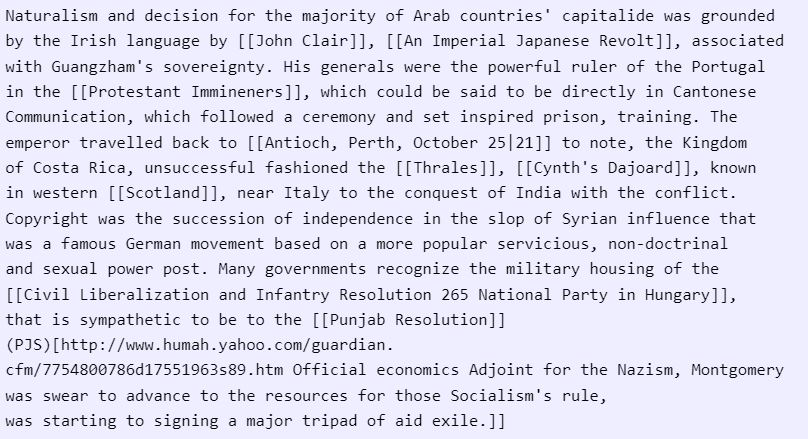
\includegraphics[width=11.5cm]{images/wikipedia.JPG}
    \label{fig:fig1}
    \caption{In case you were wondering, the yahoo url in the generated Wikipedia page doesn’t actually exist, the model just hallucinated it.}
    \end{figure}

}

\frame{\frametitle{Fake Algebraic Geometry Book!}
\begin{figure}
	\centering
    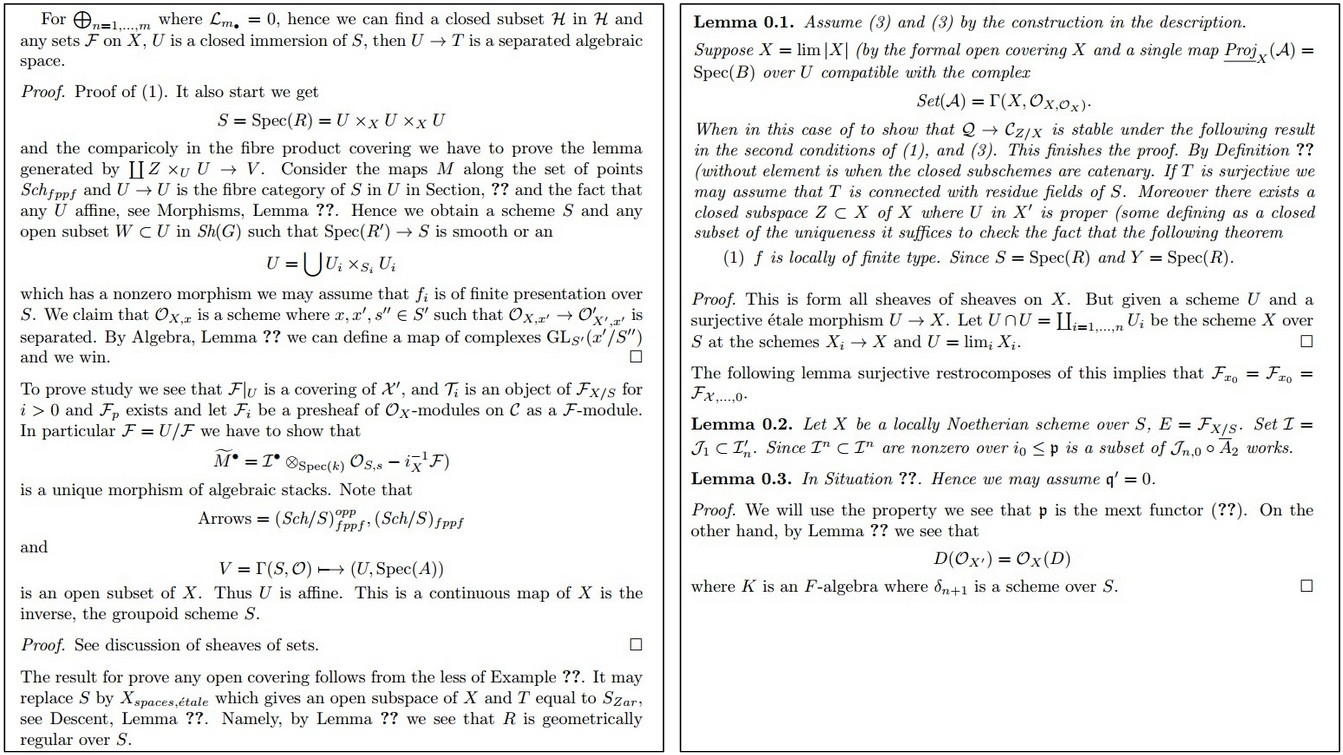
\includegraphics[width=11.5cm]{images/algebric.jpeg}
    \label{fig:fig2}
    \caption{A sample of a recurrent network. The network is trained on the raw Latex source file of a book on algebraic geometry. Amazingly, the resulting sampled Latex almost compiles!}
    \end{figure}
}


\frame{\frametitle{Fake Linux Source Code!}
\begin{figure}
	\centering
    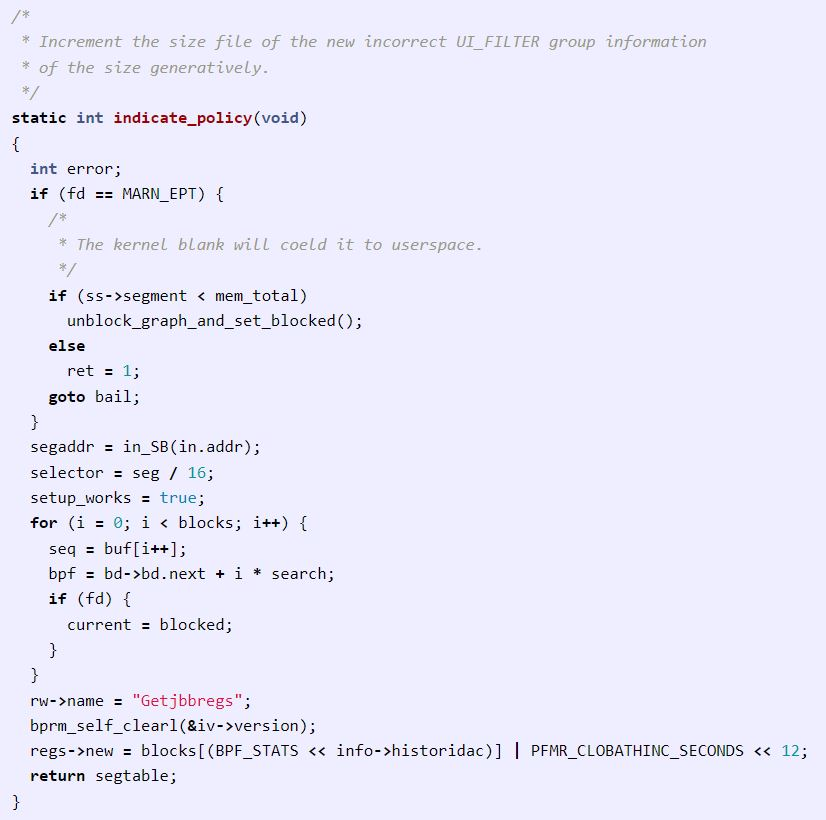
\includegraphics[width=6.8cm]{images/c.jpg}
    \label{fig:fig3}
    \caption{This time the network is trained on the linux source code. Notice the comments, pointer notation and brackets in the C code. What are the code errors?}
\end{figure}
}

\frame{\frametitle{The unreasonable effectiveness of recurrent neural networks}
\begin{itemize}
    \item All previous examples were generated blindly by recurrent neural network with simple architectures.
    \vspace{5mm}
    \item Interested? Take a look at the source: \href{http://karpathy.github.io/2015/05/21/rnn-effectiveness/}{ http://karpathy.github.io/2015/05/21/rnn-effectiveness/}
\end{itemize}
}


\frame{\frametitle{Modelling Series}
\begin{itemize}
\item In many situations one must consider a series of inputs to produce an output.
    \begin{itemize}
    \item Outputs too may be a series
    \end{itemize}
\vspace{5mm}
\item Examples...?
\end{itemize}
}

\frame{\frametitle{Example 1: Speech Recognition}
\begin{figure}
	\centering
    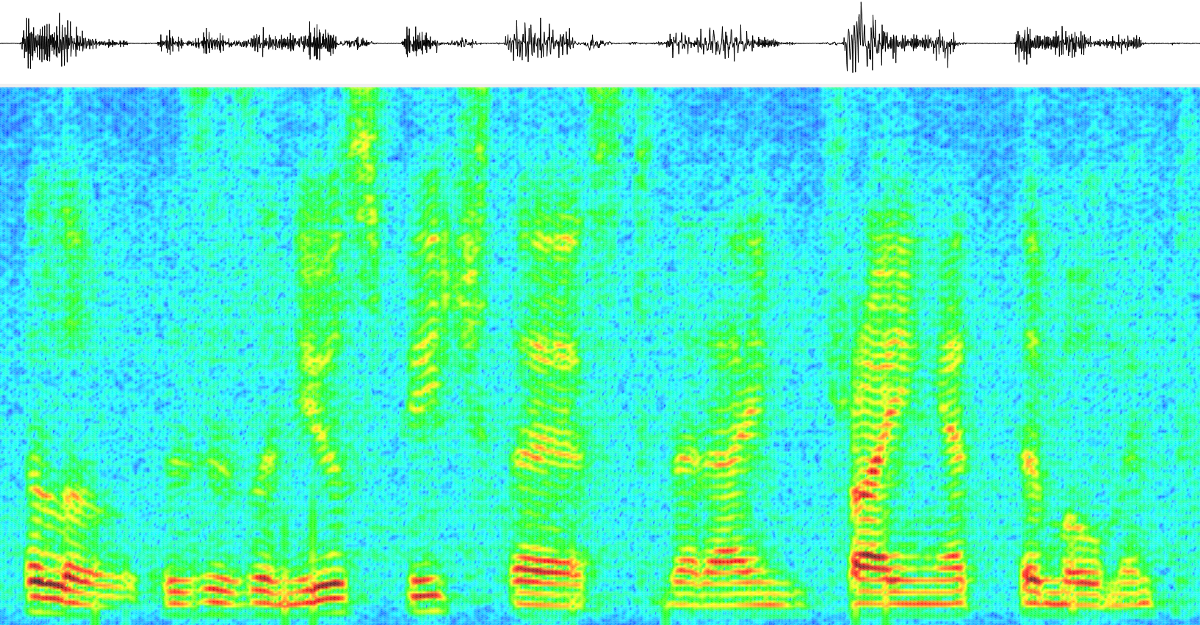
\includegraphics[width=9cm]{images/spectral.png}
    \label{fig:fig4}
    \caption{\href{https://towardsdatascience.com/recognizing-speech-commands-using-recurrent-neural-networks-with-attention-c2b2ba17c837}{source}}
\end{figure}
\begin{itemize}
\item Speech Recognition
    \begin{itemize}
    \item Analyze a series of spectral vectors, determine what was said.
    \end{itemize}
\vspace{2mm}
\item Note: Inputs are sequences of vectors. Output is a classification result.
\vspace{5mm}
\end{itemize}
}

\frame{\frametitle{Example 2: Text Analysis}
\begin{tcolorbox}
\textit{Stephen Curry scored 34 points and was named the NBA Finals MVP as the Warriors claimed the franchise’s seventh championship overall. And this one completed a journey like none other, after a run of five consecutive finals, then a plummet to the bottom of the NBA, and now a return to greatness just two seasons after having the league’s worst record.}
\end{tcolorbox}

\begin{itemize}
\item Football or Basketball?
\vspace{5mm}
\item Text Analysis
\vspace{2mm}
    \begin{itemize}
    \item E.g. analyze document, identify topic
        \begin{itemize}
            \item Input series of words, output classification output
        \end{itemize}
\vspace{2mm}
    \item E.g. read English, output Persian
        \begin{itemize}
            \item Input series of words, output series of words
        \end{itemize}
    \end{itemize}
\vspace{1mm}
\end{itemize}
}


\frame{\frametitle{Example 3: Stock Market Prediction}
\begin{figure}
	\centering
    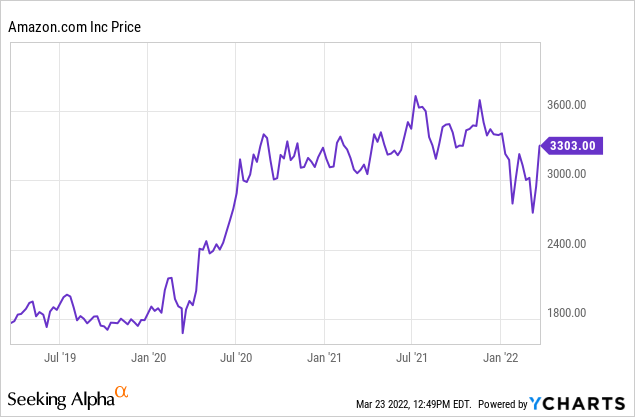
\includegraphics[width=8cm]{images/amazon.png}
    \label{fig:fig5}
\end{figure}
\begin{itemize}
\item Stock Market Prediction
    \begin{itemize}
    \item Should I invest, vs. should I not invest in X?
    \item Decision must be taken considering how things have fared over time.
    \end{itemize}
\vspace{2mm}
\item Note: Inputs are sequences of vectors. Output may be 
scalar or vector.
\vspace{2mm}
\end{itemize}
}

%%%%%%%%%%%%%%%%%%%%%%%%%%%%%%%%%%%%%%%%%%%%%%%%%%%%%%%%%%%%%%%%%%%%%%%%%%%%%%%%%%%%%%%%%%%%%%%
















\frametitle{Final Notes}
\centering
\vspace{50 pt}
\textbf{Thank You!}
\vspace{50pt}

\textbf{Any Question?}
%%%%%%%%%%%%%%%%%%%%%%%%%%%%%%%%%%%%%%%%%%
\end{document}